\subsection{Aufgabe 1: (HTML)}
\label{sec:Aufgabe1}
\begin{enumerate}[label=\alph*)]
    \item Was ist ein Pseudoelement? (\textbf{multiple chioce})
    \item Wie sehen Kommentare in HTML? (\textbf{multiple chioce})
    \item ??? (\textbf{multiple chioce})
    \item Wie sieht der zugehörige HTML-Code aus? \\
        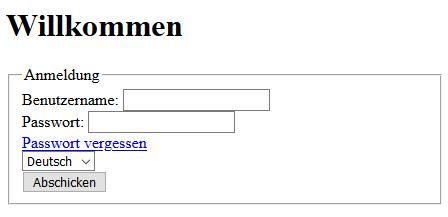
\includegraphics[width=15cm]{img/klausur.JPG}
        \begin{enumerate}[label=\arabic*.]
            \item Benutzername ist max. 80 Zeichen lang und muss immer angegeben werden.
            \item Passwort soll nicht lesbar sein.
            \item Passwort vergessen leitet nach /passwortzuruecksetzen weiter.
            \item Standardsprache Deutsch
            \item Das Formular soll an /auswertung.php geschickt werden und mit \$\_POST ausgelesen werden können.
         \end{enumerate}
    \item Nennen Sie 4 Statuscodes samt Bedeutung.
    \item Nennen Sie 4 HTTP Methoden samt Bedeutung.
\end{enumerate}